\chapter{无失真信源编码：从前缀码到 Huffman}

\section{编码问题的完整定义}

设信源符号 $X$ 取值于有限字母表 $\mathcal X=\{x_1,\dots,x_m\}$，概率为 $p_i=\Prb[X=x_i]$。二元变长码是映射
\[
C:\mathcal X\to\{0,1\}^*,
\]
其中 $\{0,1\}^*$ 表示所有有限二进制串。记码字长度为 $\ell_i=|C(x_i)|$，平均码长为
\[
L(C)=\sum_{i=1}^m p_i\ell_i.
\]

几个常被混用的概念必须分开：
\begin{description}
  \item[非奇异（nonsingular）] 不同源符号映到不同码字；
  \item[唯一可译（uniquely decodable）] 任意有限源序列连接后的比特串只能被解成唯一源序列；
  \item[前缀码（prefix-free）] 没有码字是另一码字的前缀；
  \item[瞬时码（instantaneous）] 从左到右读到一个码字结尾时即可立即输出符号，不必等待后续比特。
\end{description}
二元前缀码与瞬时码是同一类。前缀码一定唯一可译，但唯一可译码未必前缀无关；非奇异也远弱于唯一可译。

\begin{example}[非奇异但不可唯一译]
取 $C(a)=0,C(b)=01,C(c)=10$。码字互不相同，但串 $010$ 既可译为 $ac$，也可译为 $ba$，所以不是唯一可译码。
\end{example}

\section{前缀码与二叉树}

把比特 0/1 看成从根节点向左/右走一步。每个码字对应一条根到节点的路径。前缀码要求所有码字都位于叶节点：如果某码字对应内部节点，它就会成为更长码字的前缀。

\begin{center}
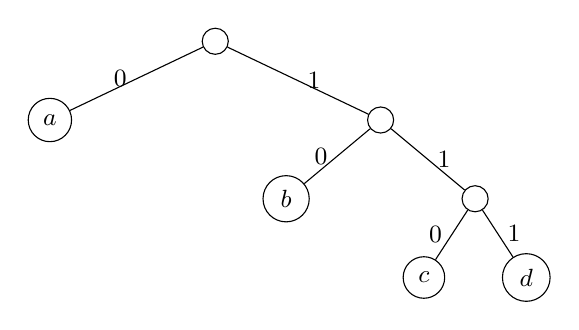
\begin{tikzpicture}[
  level distance=10mm,
  level 1/.style={sibling distance=42mm},
  level 2/.style={sibling distance=24mm},
  level 3/.style={sibling distance=13mm},
  every node/.style={font=\small}
]
\node[circle,draw] {}
 child {node[circle,draw] {$a$} edge from parent node[left] {0}}
 child {node[circle,draw] {}
   child {node[circle,draw] {$b$} edge from parent node[left] {0}}
   child {node[circle,draw] {}
     child {node[circle,draw] {$c$} edge from parent node[left] {0}}
     child {node[circle,draw] {$d$} edge from parent node[right] {1}}
     edge from parent node[right] {1}}
   edge from parent node[right] {1}};
\end{tikzpicture}
\end{center}
这棵树对应码字 $0,10,110,111$，码长为 $1,2,3,3$。

\section{Kraft--McMillan 不等式}

\begin{theorem}[Kraft 不等式]
若存在码长为 $\ell_1,\dots,\ell_m$ 的二元前缀码，则
\[
\sum_{i=1}^m 2^{-\ell_i}\le1.
\]
反过来，只要一组正整数码长满足该不等式，就存在具有这些码长的二元前缀码。
\end{theorem}

\begin{proof}[树的证明]
取 $L=\max_i\ell_i$。深度为 $\ell_i$ 的叶节点覆盖深度 $L$ 上的 $2^{L-\ell_i}$ 个后代。前缀无关保证这些后代集合互不相交，因此
\[
\sum_i2^{L-\ell_i}\le2^L.
\]
两边除以 $2^L$ 得必要性。充分性可按码长从短到长贪心分配尚未被占用的叶节点；Kraft 和不超过 1 保证每一步都有位置。
\end{proof}

对唯一可译码，更一般的 McMillan 不等式仍给出同样的必要条件。因此，在最小化平均码长时，限制到前缀码不会损失最优值。

\begin{intuitionbox}
$2^{-\ell_i}$ 可以理解为码字在无限二叉树边界上占据的“份额”。短码字占据更大的子树，所以不能给太多符号同时分配短码字。
\end{intuitionbox}

\section{熵与平均码长的基本界}

\begin{theorem}[无失真一符号编码界]
对任意唯一可译二元码，
\[
L\ge H(X).
\]
并且存在前缀码满足
\[
H(X)\le L < H(X)+1.
\]
\end{theorem}

\begin{proof}[下界]
令 $K=\sum_i2^{-\ell_i}\le1$，定义分布
\[
q_i=\frac{2^{-\ell_i}}{K}.
\]
直接计算可得
\[
D_{\mathrm{KL}}(P\|Q)=L-H(X)+\log_2K.
\]
因此
\[
L-H(X)=D_{\mathrm{KL}}(P\|Q)-\log_2K\ge0.
\]
\end{proof}

\begin{proof}[上界]
取 Shannon 码长
\[
\ell_i=\left\lceil-\log_2p_i\right\rceil.
\]
则 $2^{-\ell_i}\le p_i$，所以 Kraft 和不超过 1，存在相应前缀码。同时
\[
\ell_i<-\log_2p_i+1,
\]
对 $p_i$ 加权求和即得 $L<H(X)+1$。
\end{proof}

\begin{warningbox}
$L\ge H(X)$ 是平均码长的结论，不是说每个符号码长都至少为其自信息，也不是说任意一个文件都一定能压缩。整数码长造成的一符号冗余可以通过分块编码摊薄。
\end{warningbox}

\section{Huffman 算法}

Huffman 算法在所有二元前缀码中最小化平均码长：
\begin{enumerate}
  \item 选择概率最小的两个符号；
  \item 把它们合并为概率之和的新节点；
  \item 在缩小后的字母表上重复；
  \item 逆序展开合并树，左右边分别标 0/1。
\end{enumerate}

\begin{example}[完整 Huffman 计算]
仍取 $p=(1/2,1/4,1/8,1/8)$：
\[
1/8+1/8\to1/4,
\qquad
1/4+1/4\to1/2,
\qquad
1/2+1/2\to1.
\]
得到码长 $1,2,3,3$，平均码长
\[
L=\frac12+\frac12+\frac38+\frac38=1.75\bits=H(X).
\]
这里恰好等于熵，是因为所有概率都是 $2$ 的负整数次幂。
\end{example}

\subsection{为什么贪心是最优的}

最优性证明包含两个关键事实：
\begin{enumerate}
  \item 存在一棵最优前缀树，使概率最小的两个符号位于最深层且互为兄弟；这是通过交换叶节点而不增大平均码长得到的；
  \item 把这两个兄弟合并为一个伪符号后，原问题的最优树对应缩小问题的最优树，否则可替换为更优子树并产生矛盾。
\end{enumerate}
这正是贪心选择性质与最优子结构。

若使用最小堆，Huffman 建树时间为 $O(m\log m)$。编码和解码时间还取决于消息长度和树/码表表示。

\section{分块编码与渐近信源编码定理}

对独立同分布信源 $X_1,X_2,\dots$，把长度 $n$ 的块 $X^n$ 当作一个大符号。直接应用上一节的界：
\[
H(X^n)\le L_n<H(X^n)+1.
\]
因为独立同分布给出 $H(X^n)=nH(X)$，故每个源符号的平均码长满足
\[
H(X)\le\frac{L_n}{n}<H(X)+\frac1n.
\]
这说明整数码长造成的每符号冗余可随块长趋于无穷而消失。

\subsection{典型集与 AEP}

定义弱典型集
\[
A_\epsilon^{(n)}=
\left\{x^n:
\left|-\frac1n\log_2p(x^n)-H(X)\right|\le\epsilon
\right\}.
\]
渐近等概率性质（AEP）说明：对任意 $\epsilon>0$，
\[
\Prb[X^n\in A_\epsilon^{(n)}]\to1.
\]
典型序列的概率约为 $2^{-nH(X)}$，典型集大小约为 $2^{nH(X)}$。更精确地，当 $n$ 足够大时，
\[
(1-\epsilon)2^{n(H-\epsilon)}
\le |A_\epsilon^{(n)}|
\le 2^{n(H+\epsilon)}.
\]

\begin{theorem}[几乎无失真固定长度信源编码]
对独立同分布有限字母表信源：
\begin{itemize}
  \item 若码率 $R>H(X)$，存在长度 $n$ 的固定长度块码，使错误概率趋于 0；
  \item 若 $R<H(X)$，错误概率不能趋于 0。
\end{itemize}
\end{theorem}

\begin{proof}[可达性骨架]
给每个典型序列分配唯一索引，非典型序列统一报错。典型集大小至多
\[
2^{n(H+\epsilon)}.
\]
所以当 $R>H+\epsilon$ 时有足够的 $2^{nR}$ 个索引。错误只在非典型事件上发生，其概率趋于 0。
\end{proof}

\begin{proof}[逆定理直觉]
码率 $R$ 的固定长度码最多区分 $2^{nR}$ 个序列，而高概率质量分散在约 $2^{nH}$ 个典型序列上。若 $R<H$，可唯一表示的典型序列只占指数级变小的一部分，无法让错误概率消失。
\end{proof}

\section{三类结论不要混在一起}

\begin{center}
\begin{tabularx}{\textwidth}{lXXX}
\toprule
情形 & 是否允许错误 & 主要对象 & 结论\\
\midrule
一符号变长码 & 不允许 & 平均整数码长 & $H\le L<H+1$\\
分块变长码 & 不允许 & 每符号平均码长 & $H\le L_n/n<H+1/n$\\
固定长度块码 & 允许小错误 & 码率与错误概率 & $R>H$ 可使错误趋零\\
\bottomrule
\end{tabularx}
\end{center}

\section{小结与验收}

\begin{checkpointbox}
\begin{enumerate}
  \item 给出“非奇异、唯一可译、前缀码”的包含关系和一个反例；
  \item 用二叉树证明 Kraft 不等式；
  \item 对概率 $(0.4,0.3,0.2,0.1)$ 手工运行 Huffman 算法并计算平均码长；
  \item 解释 $H\le L<H+1$ 中的 1 从哪里来，分块为何能摊薄它；
  \item 区分无错变长编码定理与允许小错误的固定长度信源编码定理。
\end{enumerate}
\end{checkpointbox}
